\documentclass[appendixprefix,a4paper]{scrreprt}
\usepackage{amsmath,amsfonts,amssymb}
\usepackage{mathpazo}
\usepackage[utf8]{inputenc}
\usepackage[Bjornstrup]{fncychap}
\usepackage{graphicx}
\usepackage{hyperref}
\usepackage{booktabs}
\usepackage[font={small,up},labelfont=bf,hang]{caption}
\usepackage[font={small,up},labelfont=rm]{subfig}
\usepackage{todonotes}

\graphicspath{{./images/}}

\title{Cindy3D Project Documentation\vspace*{1cm}\\

\includegraphics[width=\textwidth]{title}}
\author{Matthias Reitinger \and Jan Sommer}

\begin{document}
\maketitle

\newpage

\tableofcontents

\newpage

\chapter{Project overview}

\section{Cinderella \& CindyScript}

\emph{Cinderella} is a dynamic geometry software created by Ulrich Kortenkamp and Jürgen Richter-Gebert. One of its key features is the embedded functional scripting language \emph{CindyScript}. It enables users of \emph{Cinderella} to interact with geometric constructions in a programmatic way. Among others, \emph{CindyScript} provides a rich set of methods for drawing two-dimensional geometry. However the display of three-dimensional objects is cumbersome, as one would have to fall back on the 2D drawing methods and implement algorithms like perspective projection and hidden surface removal by hand.

The recent release of \emph{Cinderella 2.6} provides a new plug-in interface. 
This allows programmers to write \emph{Java} libraries which expose 
\emph{CindyScript} methods that can in turn be called from inside 
\emph{Cinderella} constructions.

\section{Cindy3D}

In this context the \emph{Cindy3D} project was born. The need for 3D drawing 
functionality in \emph{Cinderella} was in fact one of the main reasons to 
create the new plug-in interface. The first version of \emph{Cindy3D} was 
developed when the plug-in interface was still in a preliminary stage.

The main goals for \emph{Cindy3D} were as follows:
\begin{itemize}
\item Free placement of geometric primitives in 3D space: points, segments, 
lines, rays, polygons, circles, spheres, and quad meshes
\item Control over material parameters: color, shininess, transparency
\item Customization of scene parameters: background, lights and camera
\item High-quality rendering
\item Interactive exploration of the scene
\item User-friendly \emph{CindyScript} interface:
	\begin{itemize}
	\item Useful set of functions which are exposed to the user
	\item Function names similar to the existing 2D drawing functions (if a 
corresponding function exists)
	\item Sensible default parameters
	\end{itemize}
\item Support for all major platforms on which \emph{Cinderella} runs: 
Windows, Mac OS X, Linux
\item Hardware acceleration support
\end{itemize}

\section{Results}
We are confident that we met all the main goals as stated in the previous 
section. The following screen shots directly taken from a \emph{Cindy3D} 
session illustrate the capabilities of the plugin. The \emph{CindyScript} 
source code used to generate these images can be found in appendix 
\ref{chap:source}. For details on what can be done with \emph{Cindy3D}, please 
refer to the user documentation in chapter \ref{chap:userdoc}.

\subsection{Primitive types}

\begin{figure}
\centering
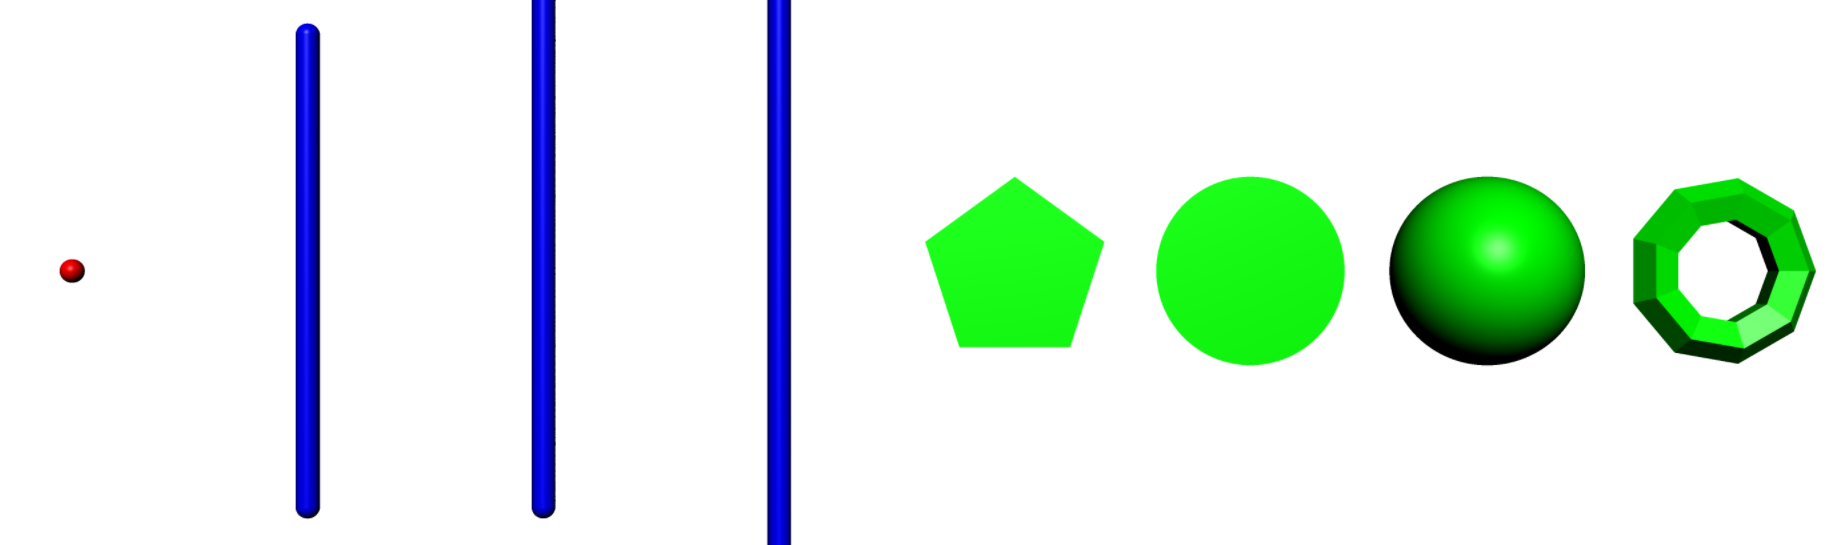
\includegraphics[width=\textwidth]{primitives}
\caption[Supported primitives]{Supported primitives. Point, segment, ray, 
line, polygon, circle, sphere, and quad mesh.}
\label{fig:primitives}
\end{figure}

Figure \ref{fig:primitives} shows the primitive types we support. 
They can be combined to produce more complex geometry like in the image on 
the title page, which consists of a thousand intersecting spheres. The quad 
mesh supports three different topologies (circular, cylindrical, toroidal) 
only one of which is shown in the figure.

\subsection{Material parameters}

\begin{figure}
\centering
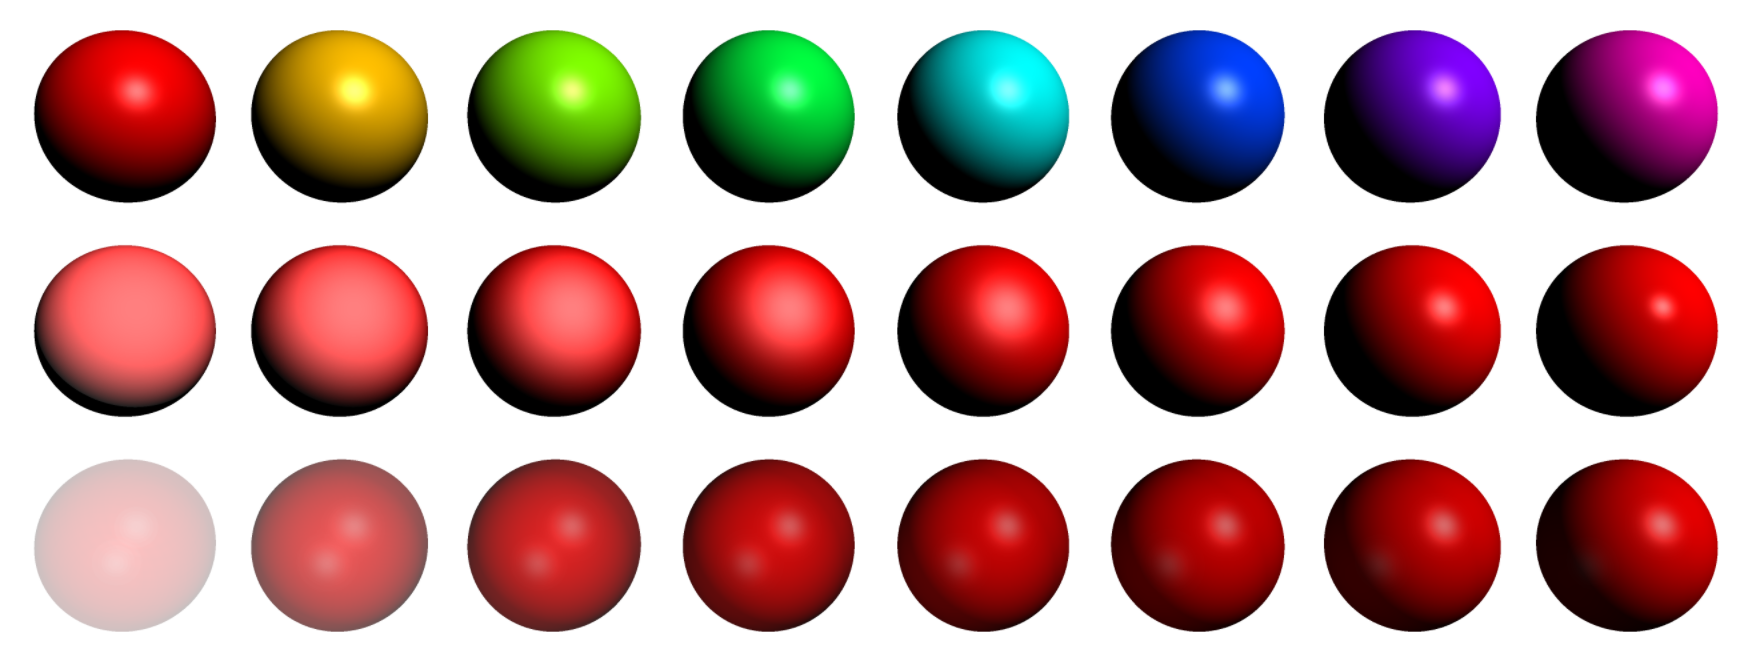
\includegraphics[width=\textwidth]{material}
\caption[Material parameters]{Material parameters. Variations in color (first 
row), shininess (second row), and transparency (third row).}
\label{fig:material}
\end{figure}

Figure \ref{fig:material} illustrates the different material parameters which 
can be specified per primitive. The user can either set default parameters or 
define the parameters in each draw command with \emph{CindyScript}'s modifier 
syntax. It's also possible to mix and match both methods and set a default 
material, overriding it with modifiers in some special cases.

\subsection{Scene parameters}

\begin{figure}
\centering
\subfloat[Default]{

\includegraphics[width=0.24\textwidth]{title}
\label{fig:scene:default}
}
\subfloat[Background]{
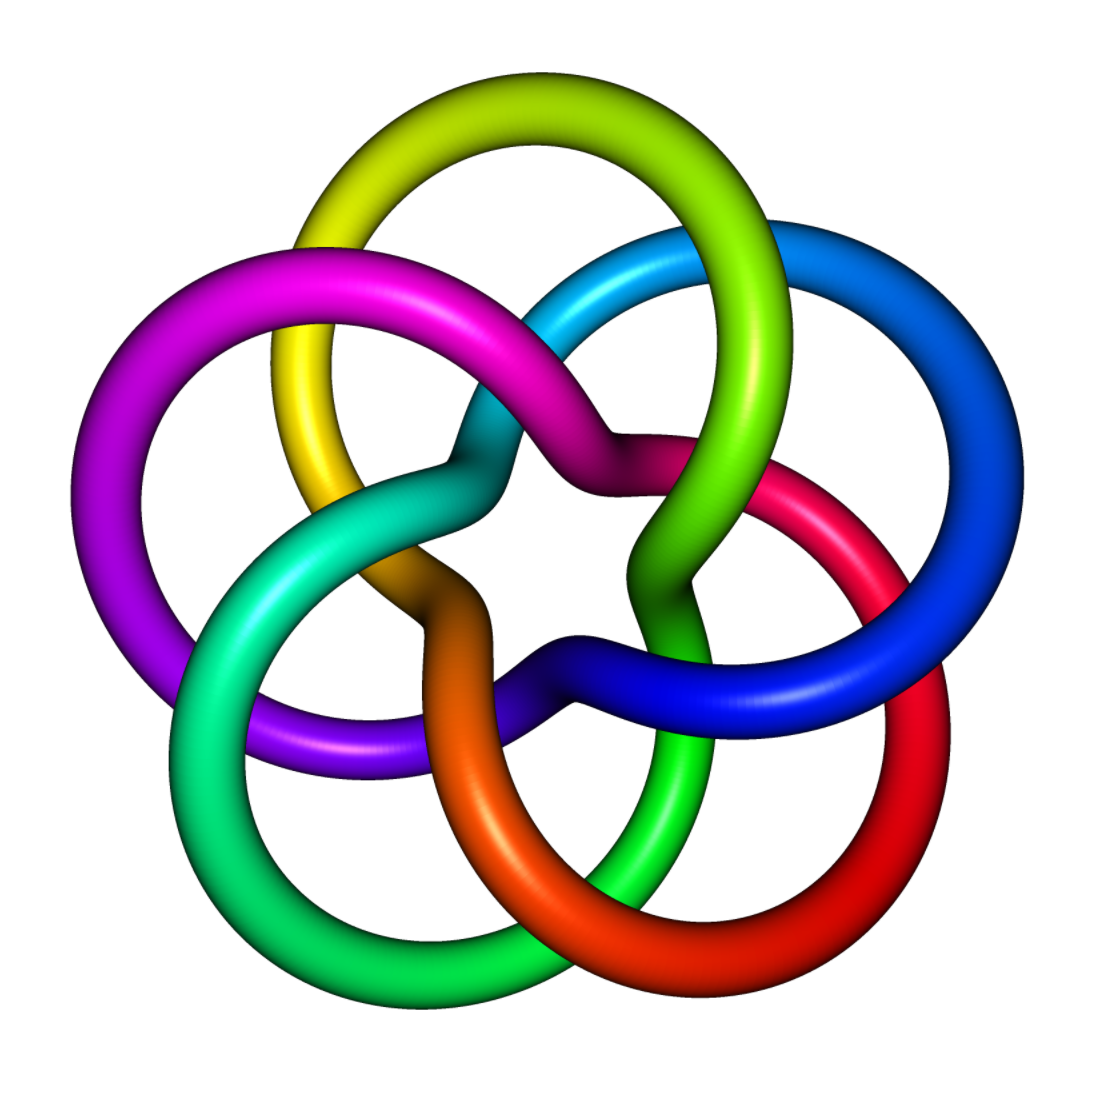
\includegraphics[width=0.24\textwidth]{scene1}
\label{fig:scene:background}
}
\subfloat[Lights]{

\includegraphics[width=0.24\textwidth]{scene2}
\label{fig:scene:lights}
}
\subfloat[Camera]{
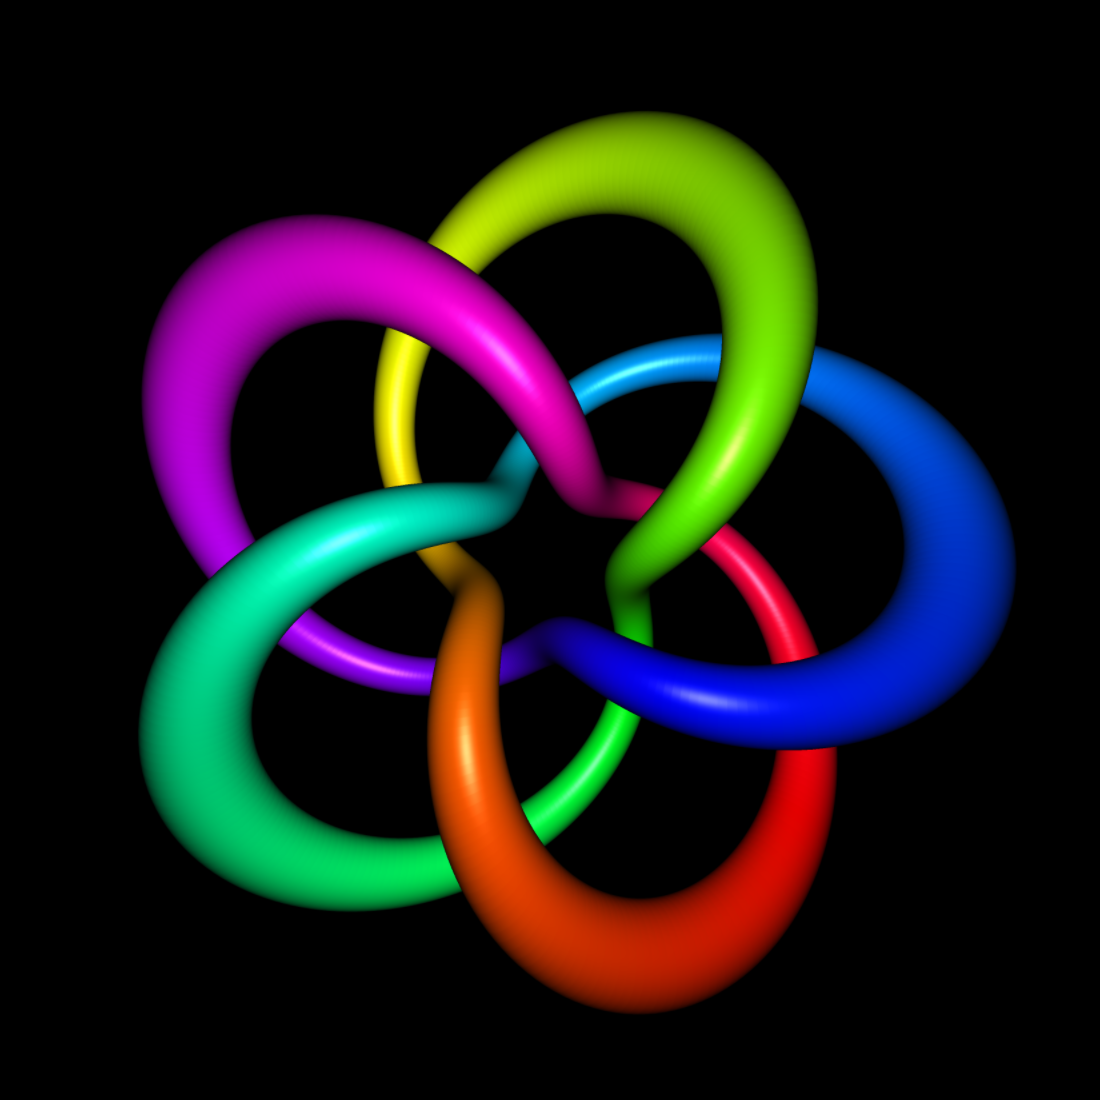
\includegraphics[width=0.24\textwidth]{scene3}
\label{fig:scene:camera}
}
\caption[Scene parameters]{Scene parameters. Changes in 
\subref{fig:scene:background} background color, \subref{fig:scene:lights} 
light setting and \subref{fig:scene:camera} camera parameters are possible.}
\label{fig:scene}
\end{figure}

In figure \ref{fig:scene} the same geometry is shown four times with different 
scene parameters. The background can be set to a new color 
(\ref{fig:scene:background}). In \ref{fig:scene:lights} the light setting has 
been changed to two directional lights coming from above (blue light) and 
below (orange light). Finally, \ref{fig:scene:camera} shows the effect of 
setting the camera's field of view to 120 degrees (the default is 45 
degrees). It is also possible to position the camera freely in 3D space.

\subsection{Rendering quality}

\begin{figure}
\centering
\subfloat[LQ, no AA]{
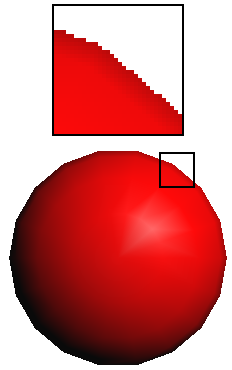
\includegraphics[width=0.24\textwidth]{quality0}
\label{fig:quality:lq}
}
\subfloat[LQ, with AA]{
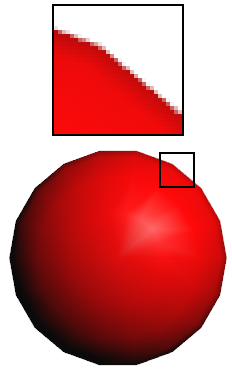
\includegraphics[width=0.24\textwidth]{quality1}
\label{fig:quality:lq-aa}
}
\subfloat[HQ, no AA]{
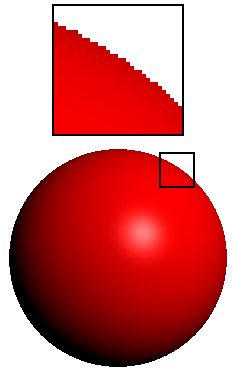
\includegraphics[width=0.24\textwidth]{quality2}
\label{fig:quality:hq}
}
\subfloat[HQ, with AA]{
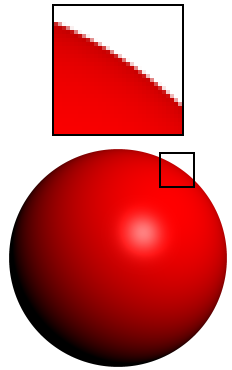
\includegraphics[width=0.24\textwidth]{quality3}
\label{fig:quality:hq-aa}
}
\caption[Rendering quality]{Rendering quality. Different quality settings with 
low-quality (LQ) or high-quality (HQ) rendering and optional anti-aliasing 
(AA).}
\label{fig:quality}
\end{figure}

The rendering quality of \emph{Cindy3D} can be adjusted depending on the 
capabilities of the user's machine. Figure \ref{fig:quality} compares 
different quality levels, ranging from the low-quality mode displaying 
triangular approximations of curved geometry (\ref{fig:quality:lq}) to 
the high-quality mode which uses ray casting to find exact intersections 
with the geometry (\ref{fig:quality:hq}). Each of the two render modes can 
optionally be enhanced by anti-aliasing techniques to alleviate jaggy borders 
on object silhouettes (\ref{fig:quality:lq-aa} and \ref{fig:quality:hq-aa}).

The high-quality mode in conjunction with anti-aliasing is able to produce 
images comparable to state of the art off-line rendering solutions at 
interactive rates. It is however more taxing on the hardware, requiring a 
fairly decent GPU to display complex scenes in the higher quality levels. The 
low-quality mode is intended for users with slower hardware and trades off 
image quality for faster rendering time.

\subsection{Interactive exploration}

The generated scene can be explored interactively by the user. The camera's 
position and orientation can be controlled with the computer mouse. It's 
possible to rotate, zoom and pan the camera to reach the camera angle you need.

\subsection{User-friendly interface}

We tried hard to make the \emph{CindyScript} interface as user-friendly and 
consistent as possible. All \emph{Cindy3D} function names end with 
\texttt{3d}, making it easy to spot \emph{Cindy3D} commands in a piece of 
code. Users already familiar with the 2D drawing functions of 
\emph{Cinderella} will notice that many functions like \texttt{color3d}, 
\texttt{size3d}, \texttt{draw3d}, \texttt{gsave3d}, etc. work just like their 
2D counterparts \texttt{color}, \texttt{size}, \texttt{draw}, 
\texttt{gsave}, etc. A comprehensive command reference is provided as part of 
this document (section \ref{sec:comref}). Additionally a user guide is 
available to help new users get up to speed (section \ref{sec:userguide}).

\subsection{Cross-platform support}

\emph{Cindy3D} has been developed with platform independence in mind and has 
been tested on all major operating systems, i.e. Windows, Mac OS X, and Linux. 
It will probably also run on other platforms, provided that \emph{Cinderella} 
supports it and \emph{OpenGL} is available for hardware acceleration.

\section{Future directions}

There are some features we would have wanted in \emph{Cindy3D}, yet didn't 
make it into this release for various reasons (like limited time or 
constraints in \emph{Cinderella} at the time of development). We hope that 
these features can be implemented in further versions of \emph{Cindy3D}:

\begin{itemize}
\item Coordinate system transformations (\texttt{translate3d}, 
\texttt{rotate3d}, \texttt{scale3d})
\item Embedding \emph{Cindy3D} into the \emph{Cinderella} drawing surface
\item Applet support
\item 2D function plots as additional primitive
\end{itemize}


\chapter{User documentation}
\label{chap:userdoc}

\section{Installation}

\begin{itemize}
\item Minimum system requirements (OpenGL version...)
\item Install guide (with screenshots?)
\end{itemize}

\section{User guide}
\label{sec:userguide}

\begin{itemize}
\item Understanding of \emph{CindyScript} is assumed
\item Scene management (begin3d, end3d)
\item Coordinate system
\item Primitive types
\item Appearance (attributes, stack)
\item Lights and shading model
\item Examples
\item Tutorial(s)?
\end{itemize}

\section{Command reference}
\label{sec:comref}

Link to HTML documentation or inline.


\chapter{Developer documentation}
\label{chap:devdoc}

\section{Technical overview}

\begin{itemize}
\item Java 6
\item Used libraries: JOGL, apache-commons-math
\item JAR packaging
\end{itemize}

\section{Design overview}

Insert fancy diagram here.
% Translation of calls from Cinderella to a library agnostic format (only types provided by Java or derivatives thereof)

\section{Rendering}

\begin{itemize}
\item Explain raytraced rendering with proxy geometry
\item Explain LOD
\end{itemize}

\section{JavaDoc}

Link to generated JavaDoc.

\appendix

\chapter{Example source code}
\label{chap:source}

\listoffigures

\end{document}
